% =====================================================================

% =====================================================================
\documentclass[11pt,a4paper]{article}
\usepackage{fontspec}
\usepackage{float}
\usepackage[a4paper,margin=2.5cm]{geometry}
\usepackage{amsmath,amssymb}
\usepackage{xcolor}
\usepackage{longtable,booktabs,array}
\usepackage{calc}
\usepackage{graphicx}
\graphicspath{{Imagenes_DCF_IR_LATEX/}}
\usepackage{hyperref}
\usepackage{fancyhdr}
\usepackage{titlesec}
\usepackage{enumitem}
\usepackage{parskip}
\usepackage{caption}
\usepackage{tabularx}
\usepackage{tikz}
\usetikzlibrary{shapes,arrows.meta,positioning,calc,fit}
\usepackage[numbers]{natbib}

\definecolor{utequeen}{RGB}{0,102,51}
\definecolor{utequegold}{RGB}{198,161,91}

\hypersetup{
	colorlinks=true,
	linkcolor=black,    % Índice y referencias internas en negro
	urlcolor=blue,      % URLs en azul
	citecolor=blue,     % Citas bibliográficas en azul
	filecolor=blue,     % Enlaces a archivos en azul
	pdftitle={Prueba Práctica Unidad IV - Ingeniería de Requisitos},
	pdfauthor={Tigasi Sampedro Paúl Alexander}
}

\titleformat{\section}
{\normalfont\Large\bfseries\color{utequeen}}
{\thesection}{1em}{}
\titleformat{\subsection}
{\normalfont\large\bfseries\color{black}}
{\thesubsection}{1em}{}
\titleformat{\subsubsection}
{\normalfont\normalsize\bfseries\color{black}}
{\thesubsubsection}{1em}{}
\titleformat{\paragraph}[block]
{\normalfont\normalsize\bfseries\itshape\color{black}}
{\theparagraph}{1em}{}
\titlespacing*{\paragraph}{0pt}{2.5ex plus 1ex minus .2ex}{1ex}

\setcounter{secnumdepth}{4}
\setcounter{tocdepth}{3}

\pagestyle{fancy}
\fancyhf{}
\fancyhead[L]{\small Ingeniería de Requisitos (ISR-401) -- Prueba Práctica Unidad IV}
\fancyhead[R]{\small UTEQ}
\fancyfoot[C]{\thepage}
\renewcommand{\headrulewidth}{0pt}
\renewcommand{\footrulewidth}{0pt}

% Evitar que las longtable se desborden del margen
\setlength{\LTleft}{0pt}
\setlength{\LTright}{0pt}

% Definición requerida por listas generadas por pandoc
\providecommand{\tightlist}{%
	\setlength{\itemsep}{0pt}\setlength{\parskip}{0pt}}

\newcommand{\repoURL}{https://github.com/ptigasis-Alexander/Pruba_Practica_UND4_Tigasi_Sampedro} % <-- reemplazar por la URL real del repositorio


\newcommand{\scanfig}[4]{%
	% #1 = nombre del archivo (ej. scan-3.jpg)
	% #2 = ancho (ej. 0.92\linewidth)
	% #3 = texto del caption
	% #4 = label
	\begin{figure}[H]
		\centering
		\IfFileExists{Imagenes_DCF_IR_LATEX/#1}{%
			\includegraphics[width=#2]{#1}%
		}{%
			\fbox{\parbox[c][6cm][c]{#2}{\centering\itshape
					Imagen no encontrada: \texttt{#1}\\[4pt]
					Colócala en \texttt{Imagenes\_DCF\_IR\_LATEX/#1} y vuelve a compilar.}}%
		}
		\caption{#3}
		\label{#4}
	\end{figure}
}

% =====================================================================
\begin{document}
	
	% ---------------------------------------------------------------
	% CARÁTULA
	% ---------------------------------------------------------------
	\begin{titlepage}
		\centering
		\vspace*{0.5cm}
		{\large\color{utequeen}\bfseries UNIVERSIDAD TÉCNICA ESTATAL DE QUEVEDO\par}
		{\large Facultad de Ciencias de la Ingeniería\par}
		{\large Carrera de Ingeniería de Software\par}
		\vspace{1.2cm}
		
		{\color{utequegold}\rule{\linewidth}{1pt}}\par\vspace{0.4cm}
		{\Huge\bfseries\color{utequeen} Prueba Práctica --- Unidad IV\par}
		\vspace{0.3cm}
		{\Large Validación, Gestión, Herramientas y Estándares de Requisitos\par}
		\vspace{0.4cm}
		{\color{utequegold}\rule{\linewidth}{1pt}}\par
		\vspace{1cm}
		
		{\large\bfseries Caso: Sistema de Gestión de Pedidos\par}
		\vspace{1.5cm}
		
		% ---- Datos de identificación ----
		\begin{tabular}{@{}p{3.6cm}p{9.5cm}@{}}
			\textbf{Asignatura:} & Ingeniería de Requisitos (ISR-401) \\[4pt]
			\textbf{Docente:} & Ing. Gleiston Guerrero, Mg. \\[4pt]
			\textbf{Estudiante:} & Tigasi Sampedro Paúl Alexander \\[4pt]
			\textbf{Modalidad:} & Individual, en clase \\[4pt]
			\textbf{Duración:} & 120 minutos \\[4pt]
			\textbf{Ponderación:} & 100 puntos (30 cuestionario + 70 desarrollo) \\[4pt]
			\textbf{Fecha:} & 11 de agosto de 2026 \\
		\end{tabular}
		
		\vspace{1.6cm}
		
		% ---- URL del repositorio en una sola línea (criterio de piso 1) ----
		\noindent\textbf{Repositorio del proyecto (URL en una sola línea):}\par
		\vspace{0.2cm}
		\begin{center}
			\fcolorbox{utequegold}{white}{\url{\repoURL}}
		\end{center}
		
		\vspace{4.2cm}
		
		% ---- Capturas del cuestionario del SGA ----
		\noindent\textbf{Captura del resumen del cuestionario (SGA):}\par
		
		\begin{figure}[H]
			\centering
			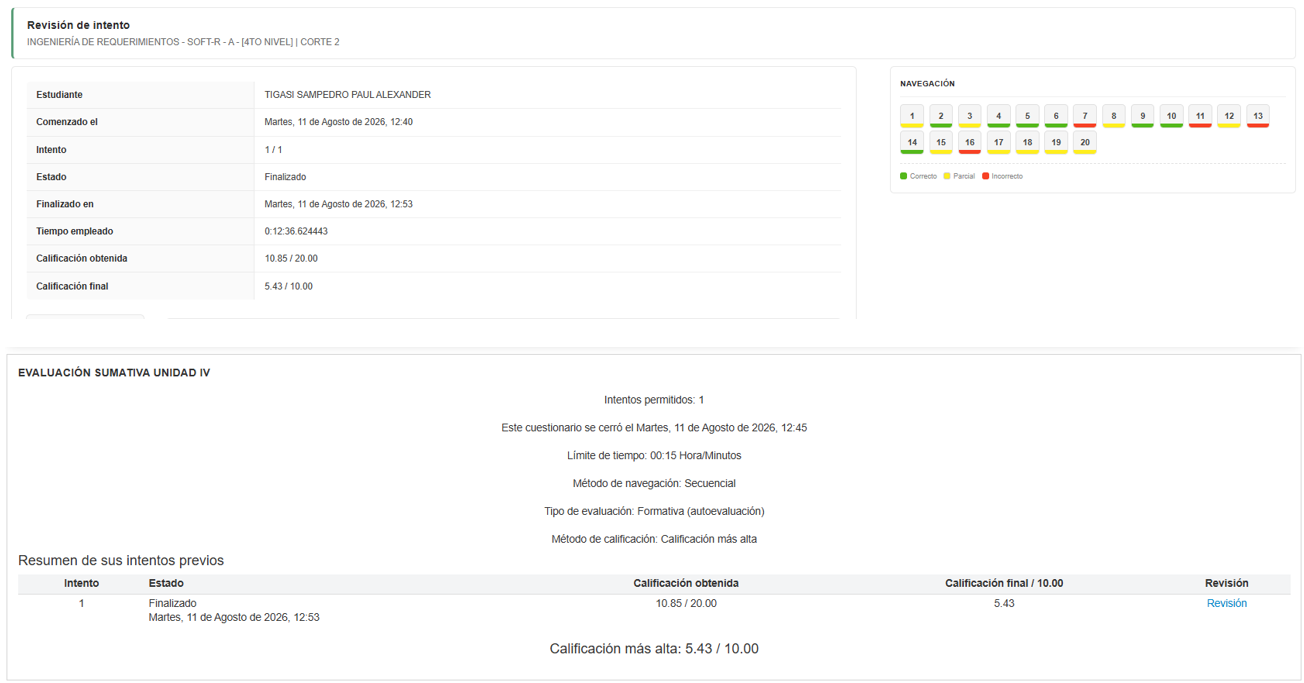
\includegraphics[width=0.85\textwidth]{ResumenCuestionarioSGA.png}
			\caption{Captura de pantalla del RESUMEN del cuestionario rendido en el SGA.}

		\end{figure}
		
		\vspace{0.6cm}
		
		\noindent\textbf{Captura de la evaluación / intento (SGA):}\par
		\vspace{0.2cm}

	\begin{figure}[H]
	\centering
	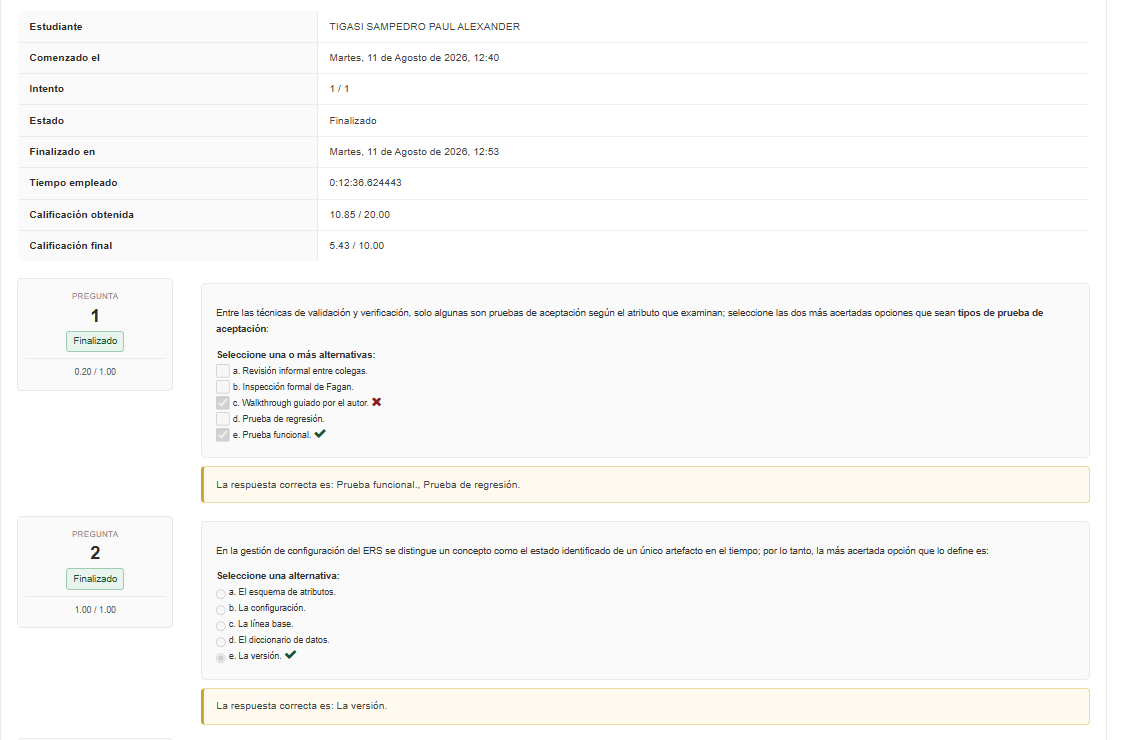
\includegraphics[width=0.85\textwidth]{CuestionarioSGA1.png}
	\caption{captura de pantalla de la EVALUACIÓN/INTENTO del cuestionario en el SGA..}
	
	\end{figure}

	\begin{figure}[H]
		\centering
		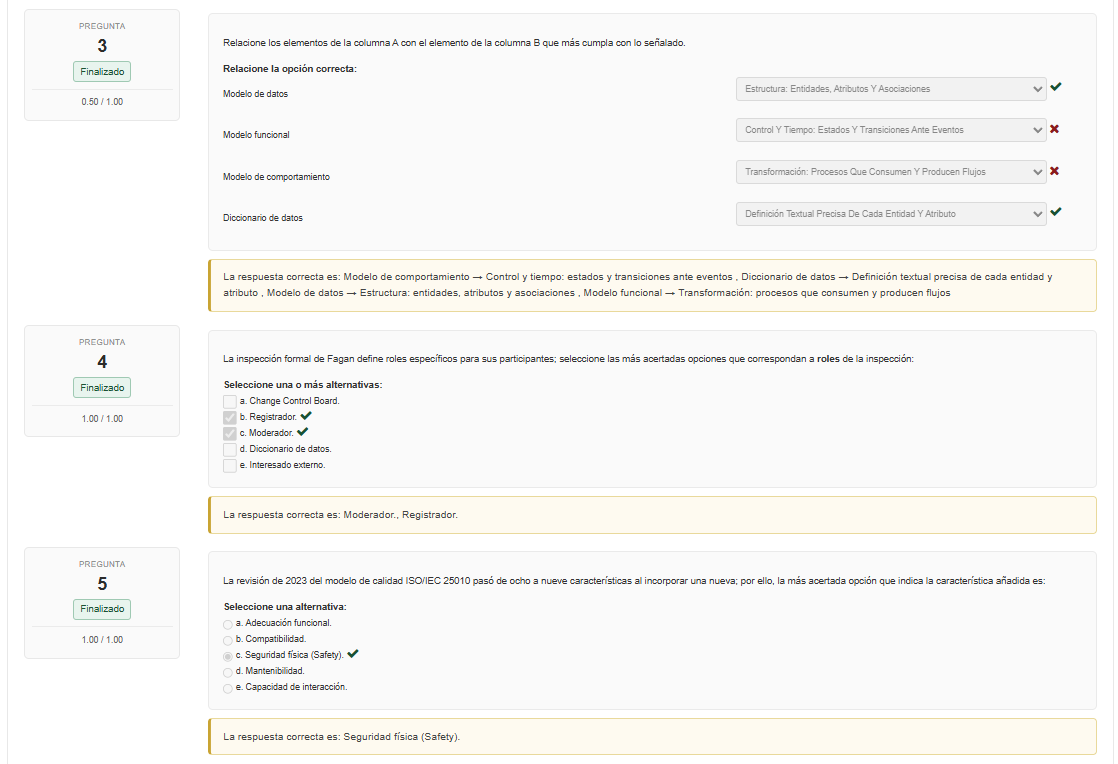
\includegraphics[width=0.85\textwidth]{CuestionarioSGA2.png}
		\caption{captura de pantalla de la EVALUACIÓN/INTENTO del cuestionario en el SGA..}
		
	\end{figure}

	\begin{figure}[H]
			\centering
			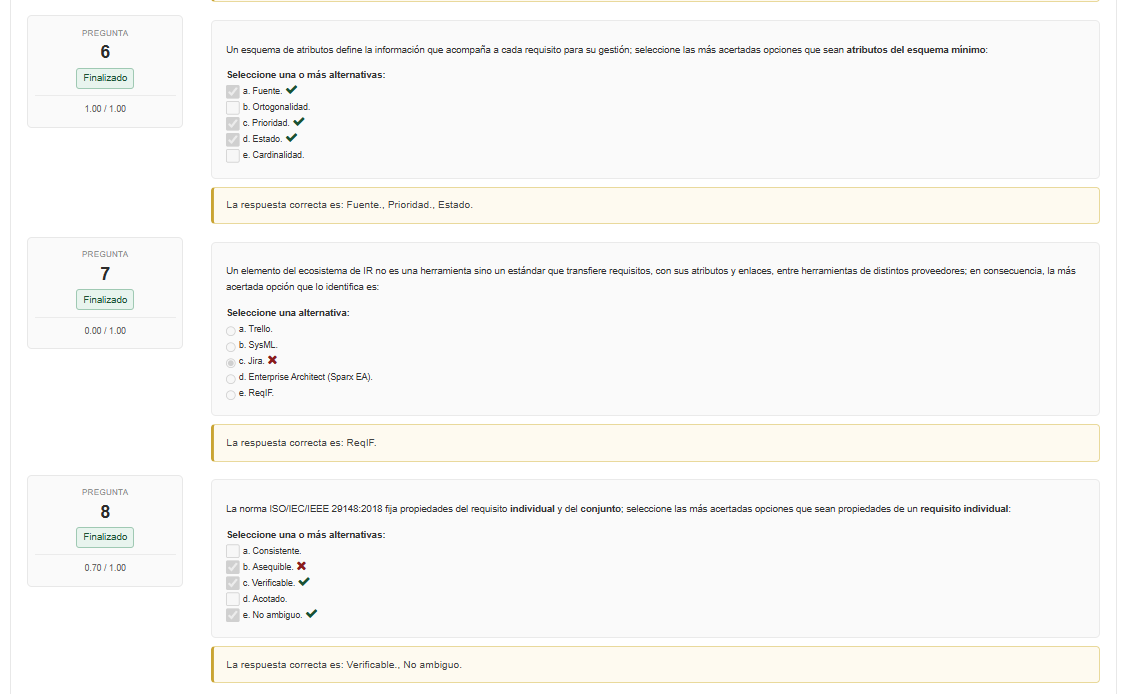
\includegraphics[width=0.85\textwidth]{CuestionarioSGA3.png}
			\caption{captura de pantalla de la EVALUACIÓN/INTENTO del cuestionario en el SGA..}
			
	\end{figure}
	
	\begin{figure}[H]
		\centering
		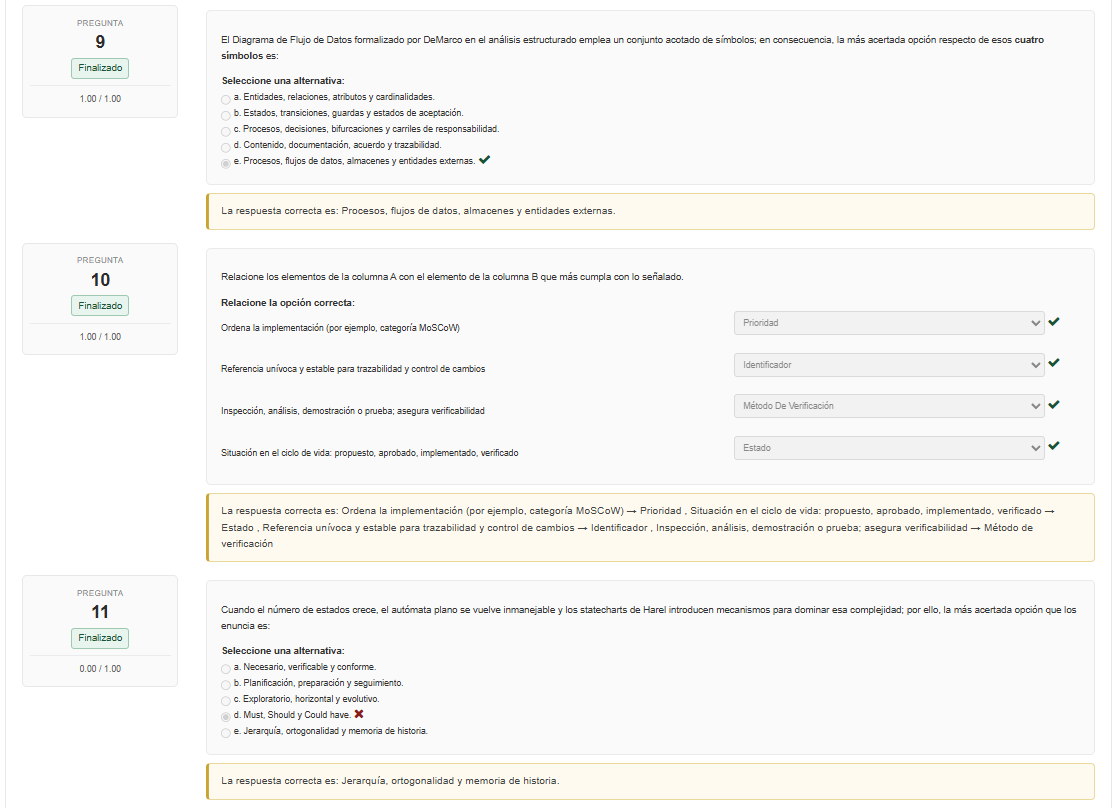
\includegraphics[width=0.85\textwidth]{CuestionarioSGA4.png}
		\caption{captura de pantalla de la EVALUACIÓN/INTENTO del cuestionario en el SGA..}
		
	\end{figure}
	
		\begin{figure}[H]
		\centering
		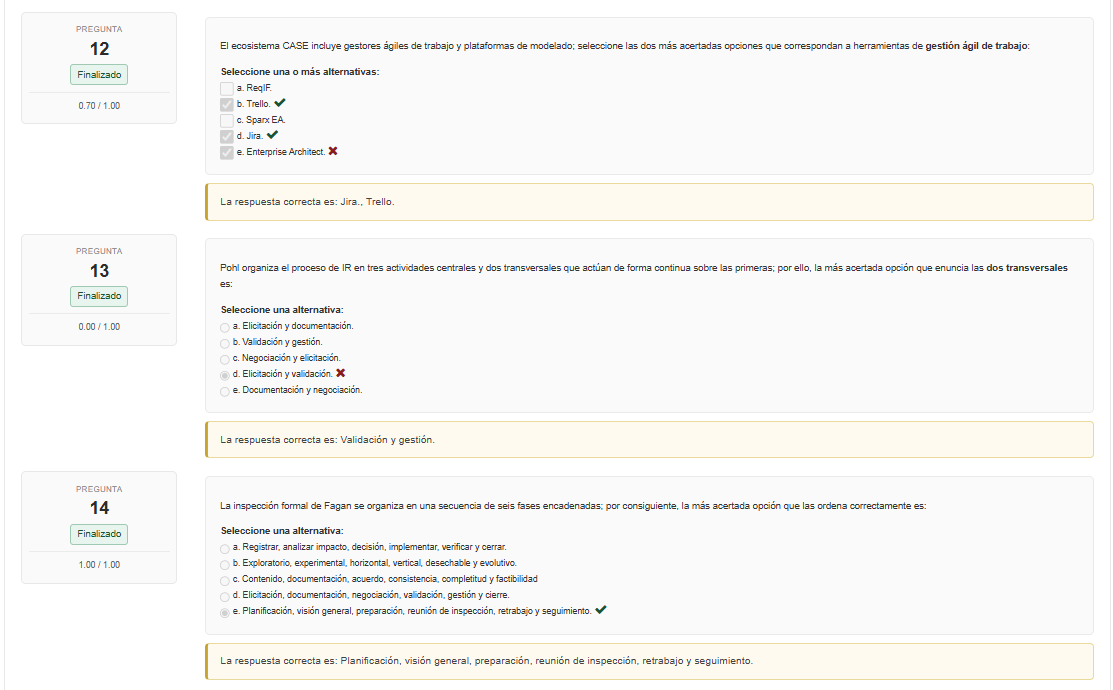
\includegraphics[width=0.85\textwidth]{CuestionarioSGA5.png}
		\caption{captura de pantalla de la EVALUACIÓN/INTENTO del cuestionario en el SGA..}
		
	\end{figure}
	
		\begin{figure}[H]
		\centering
		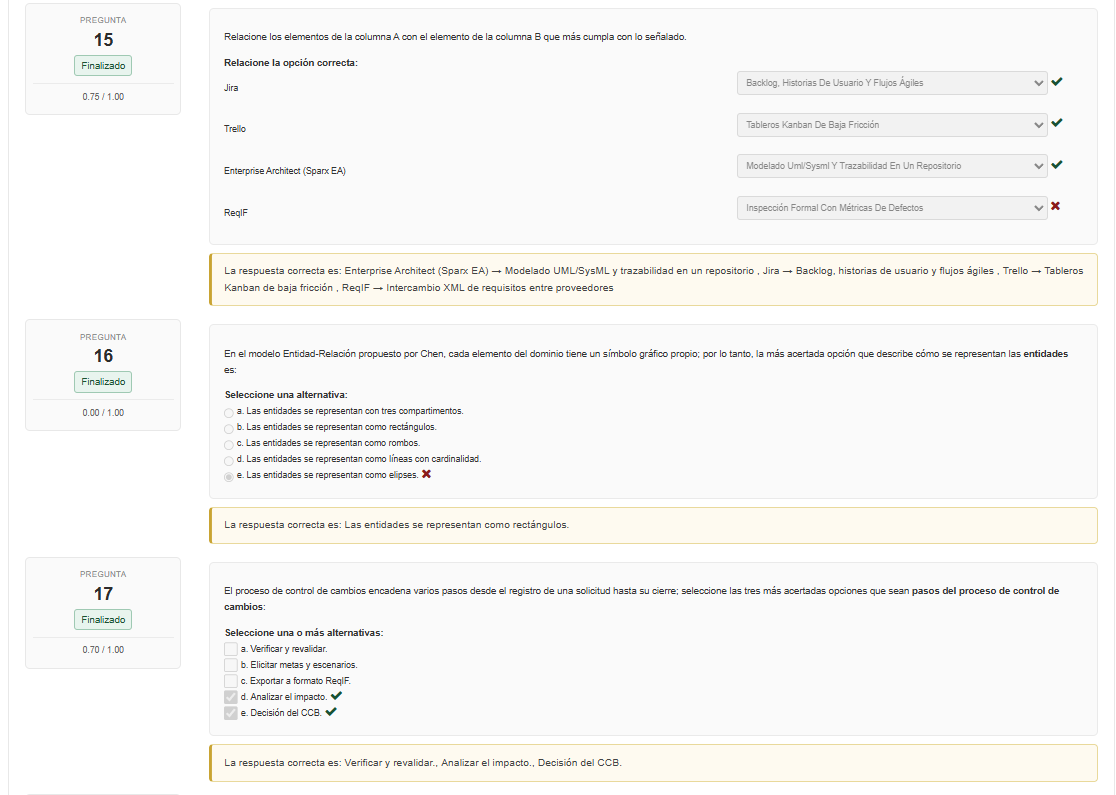
\includegraphics[width=0.85\textwidth]{CuestionarioSGA6.png}
		\caption{captura de pantalla de la EVALUACIÓN/INTENTO del cuestionario en el SGA..}
		
	\end{figure}
	
		\begin{figure}[H]
		\centering
		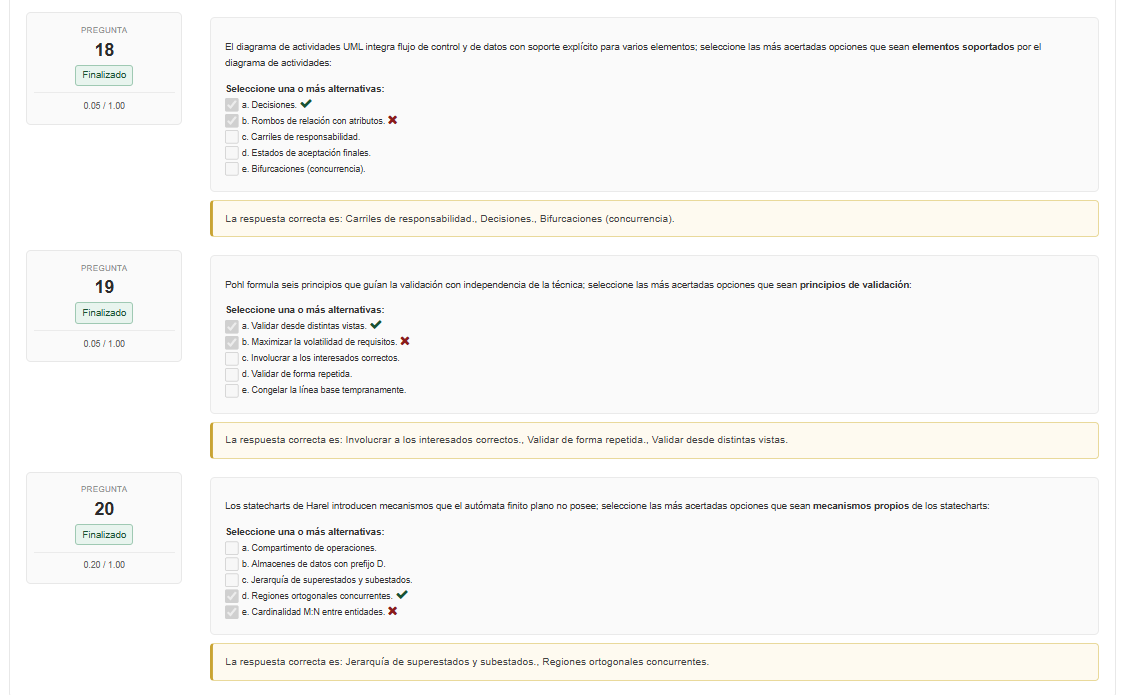
\includegraphics[width=0.85\textwidth]{CuestionarioSGA7.png}
		\caption{captura de pantalla de la EVALUACIÓN/INTENTO del cuestionario en el SGA..}
		
	\end{figure}
		
	\end{titlepage}
	
	% ---------------------------------------------------------------
	\tableofcontents
	\newpage
	
	% ---------------------------------------------------------------

	
	\newpage
	% =====================================================================
	\section{P1. Modelo de datos --- Diagrama de clases UML}
	Diagrama de clases del dominio (manuscrito original) con las clases \textbf{Cliente}, \textbf{Pedido},
	\textbf{LíneaPedido} y \textbf{Producto}, sus atributos tipados, operaciones y las multiplicidades de
	cada asociación. Los identificadores están subrayados en el original.
	
	\scanfig{DiagramaClase.png}{0.92\linewidth}{Diagrama de clases UML (P1) y diagrama de actividades (P2) ---.}{fig:p1p2}
	
	\subsection*{Transcripción de clases }
	\begin{center}
		\begin{tabular}{@{}p{5.4cm}p{5.4cm}@{}}
			\toprule
			\textbf{Cliente} & \textbf{Pedido} \\
			\midrule
			\underline{idCliente : int} & \underline{idPedido : int} \\
			nombreC : String & fechaP : Date \\
			correoC : String & totalP : Decimal \\
			+ realizarPedido() : Pedido & estadoP : String \\
			& + registrar() : void \\
			& + confirmar() : void \\
			& + anular() : void \\
			& + despachar() : void \\
			& + entregar() : void \\
			& + verificarStock() : boolean \\
			\bottomrule
		\end{tabular}
		
		\vspace{3.6cm}
		\begin{tabular}{@{}p{5.4cm}p{5.4cm}@{}}
			\toprule
			\textbf{Producto} & \textbf{LíneaPedido} \\
			\midrule
			\underline{codigoProduc : String} & \underline{idLineaPedido : int} \\
			descripcion : String & cantidad : int \\
			precio : Decimal & subtotal : Decimal \\
			stockProduc : int & + calcularSubtotal() : Decimal \\
			+ verificarStock(codigoProduc) : boolean & \\
			+ actualizarStock(cantidad, codigoProduc) : void & \\
			\bottomrule
		\end{tabular}
	\end{center}
	
	\noindent\textbf{Multiplicidades:} Cliente 1 --- 0..* Pedido; Pedido 1 --- 1..* LíneaPedido; LíneaPedido 0..* --- 1 Producto.
	
	% =====================================================================
	\section{P2. Modelo funcional --- Diagrama de actividades UML}
		
	\begin{figure}[H]
		\centering
		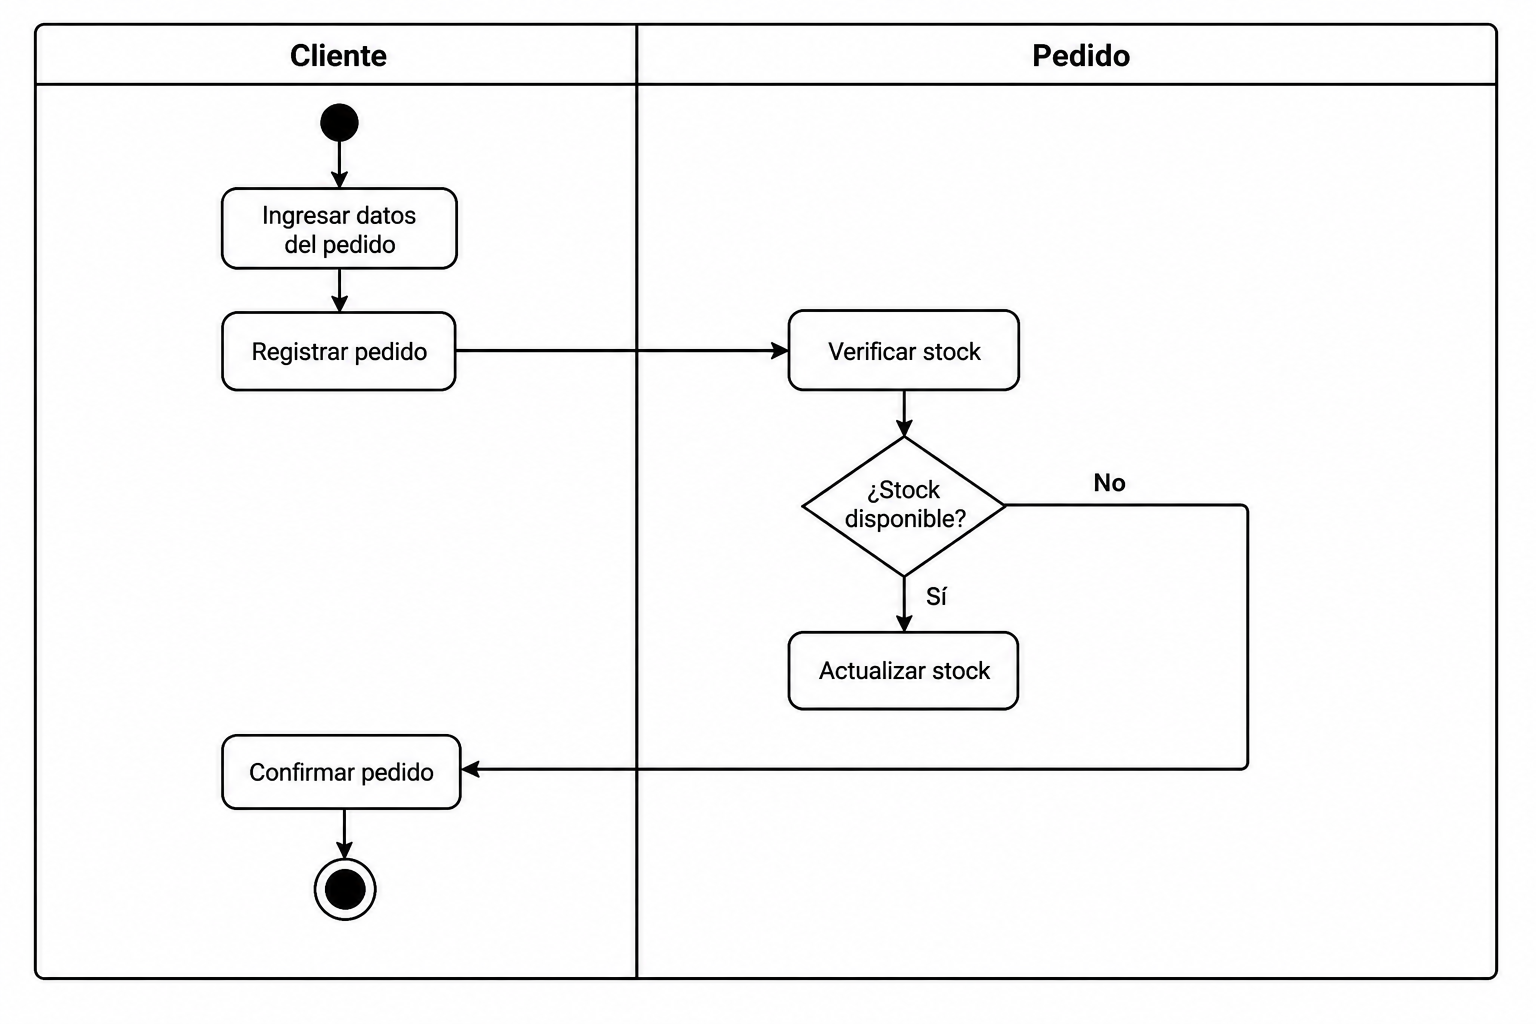
\includegraphics[width=0.85\textwidth]{diagramaActividad.png}
		\caption{Diagrama de actividad del procceso de Registrar pedido en la seccion (P2)}
		\label{fig:sd-16}
	\end{figure}
	
	Proceso ``Registrar pedido'' con carriles \emph{Cliente} y \emph{Pedido} (ver Figura~\ref{fig:p1p2}, mitad
	inferior). Nodo inicial $\to$ \emph{Ingresar datos del pedido} $\to$ \emph{Registrar pedido} $\to$
	\emph{Verificar stock} $\to$ decisión \textbf{¿Stock disponible?}: \textbf{Sí} $\to$ \emph{Actualizar stock}
	$\to$ \emph{Confirmar pedido} $\to$ nodo final; \textbf{No} $\to$ \emph{Notificar faltante}.
	
	% =====================================================================
	\section{P3. Modelo de comportamiento --- Máquina de estados UML}
	
	\scanfig{DiagramaMaquina.png}{0.92\linewidth}{Máquina de estados (P3) y tabla de consistencia (P4) --- manuscrito original.}{fig:p3p4}
	
	\subsection*{Complemento: superestado Activo y transición anular}
	El manuscrito original solo incluye Registrado $\to$ Confirmado $\to$ Enviado $\to$ Entregado. Se
	añade el estado \textbf{Cancelado} y el superestado \textbf{Activo} (que agrupa a Registrado, Confirmado
	y Enviado), del cual sale la transición \texttt{anular} hacia Cancelado.
	
	\begin{center}
		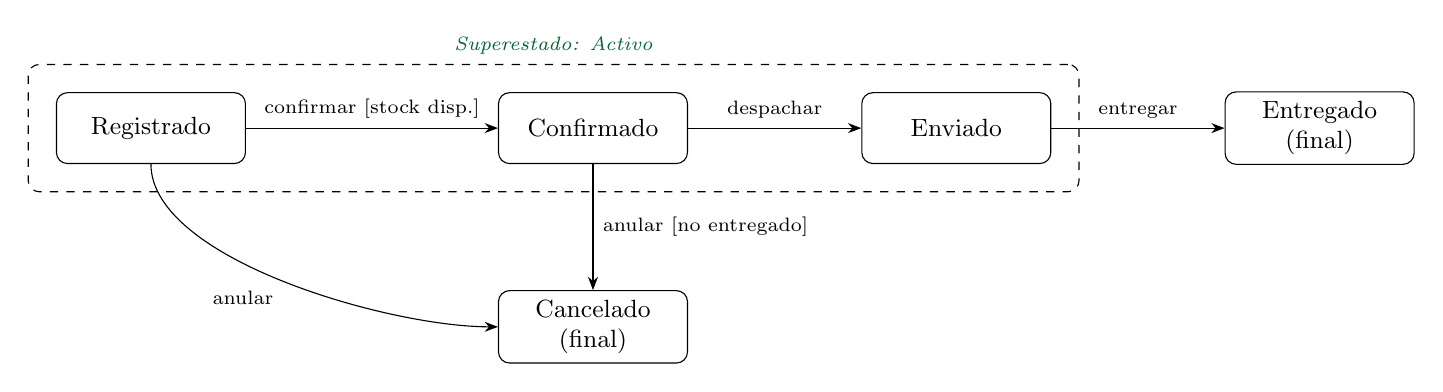
\begin{tikzpicture}[
			state/.style={draw, rounded corners, minimum width=2.4cm, minimum height=0.9cm, align=center, font=\small},
			>=Stealth
			]
			\node[state] (reg) {Registrado};
			\node[state, right=3.2cm of reg] (conf) {Confirmado};
			\node[state, right=2.2cm of conf] (env) {Enviado};
			\node[state, right=2.2cm of env] (ent) {Entregado\\(final)};
			\node[state, below=1.6cm of conf] (canc) {Cancelado\\(final)};
			
			\draw[->] (reg) -- node[above,font=\scriptsize,align=center]{confirmar [stock disp.]} (conf);
			\draw[->] (conf) -- node[above,font=\scriptsize]{despachar} (env);
			\draw[->] (env) -- node[above,font=\scriptsize]{entregar} (ent);
			\draw[->] (reg.south) .. controls +(0,-1.2) and +(-1.4,0) .. node[below left,font=\scriptsize,align=center]{anular} (canc.west);
			\draw[->] (conf) -- node[right,font=\scriptsize,align=center]{anular [no entregado]} (canc);
			
			\node[draw, dashed, rounded corners, fit=(reg)(conf)(env), inner sep=10pt, label=above:{\scriptsize\itshape\color{utequeen} Superestado: Activo}] {};
		\end{tikzpicture}
	\end{center}
	
	% =====================================================================
	\section{P4. Consistencia entre las tres perspectivas}
	Tabla cruzada evento (P3) $\to$ acción (P2) $\to$ elemento de datos (P1). Ver Figura~\ref{fig:p3p4}.
	
	\begin{center}
		\begin{tabular}{@{}lll@{}}
			\toprule
			\textbf{Evento (P3)} & \textbf{Acción (P2)} & \textbf{Elemento (P1)} \\
			\midrule
			registrar & registrar pedido & Pedido.estado \\
			confirmar & confirmar pedido & Pedido.estado \\
			despachar & despachar pedido & Pedido.estado \\
			entregar & entregar pedido & Pedido.estado \\
			anular & anular pedido & Pedido.estado \\
			verificarStock & verificar disponibilidad & Producto.stock \\
			actualizarStock & actualizar stock & Producto.stock \\
			\bottomrule
		\end{tabular}
	\end{center}
	
		\scanfig{DiagrmaMaquinaEstadoCorregido.png}{0.92\linewidth}{Máquina de estados (P3) corregido --- .}{fig:p3p12}
	
	\newpage
	% =====================================================================
	\section{P5. Especificación de requisitos con esquema de atributos}
	
	
	\begin{description}[leftmargin=1.6cm,style=nextline]
		\item[RF1 --- Registrar pedido] El sistema deberá permitir al cliente registrar un pedido con uno
		o más productos, verificando su disponibilidad antes de confirmarlo.
		\item[RF2 --- Gestionar estado del pedido] El sistema deberá permitir gestionar el estado del
		pedido mediante los estados Confirmado, Enviado, Entregado y Cancelado.
		\item[RNF1 --- Tiempo de respuesta (Eficiencia de desempeño, ISO/IEC 25010)] El sistema deberá
		procesar la solicitud de un pedido en menos de 2 segundos en al menos el 95\% de las
		operaciones bajo condiciones normales (v1.1).
		\item[RNF2 --- Protección de datos (Seguridad, ISO/IEC 25010)] El sistema deberá proteger los
		datos del cliente mediante autenticación usuario/contraseña, cifrado en tránsito (TLS 1.2+) y
		control de acceso por roles.
	\end{description}
	
	\begin{center}
		\begin{tabular}{@{}lllllll@{}}
			\toprule
			ID & Prioridad & Estado & Fuente & Estabilidad & Versión & Verificación \\
			\midrule
			RF1 & Must & Propuesto & Caso práctico & Alta & 1.0 & Prueba funcional (PA1) \\
			RF2 & Must & Propuesto & Caso práctico & Alta & 1.0 & Prueba funcional (PA2) \\
			RNF1 & Should & Propuesto & Caso práctico & Media & 1.1 & Prueba de rendimiento (PA3) \\
			RNF2 & Must & Propuesto & Caso práctico & Alta & 1.1 & Prueba de seguridad (PA4) \\
			\bottomrule
		\end{tabular}
	\end{center}
	
	% =====================================================================
	\section{P6. Priorización MoSCoW}
	Ver Figura~\ref{fig:p5p6}.
	\begin{center}
		\begin{tabularx}{\linewidth}{@{}llX@{}}
			\toprule
			Requisito & Categoría & Justificación \\
			\midrule
			RF1 & Must & Sin registrar pedidos el sistema no cumple su objetivo. \\
			RF2 & Must & Es necesario controlar el ciclo de vida del pedido. \\
			RNF1 & Should & La rapidez importa, pero el sistema puede operar con menor rendimiento temporalmente. \\
			RNF2 & Must & El caso exige proteger los datos personales del cliente. \\
			\bottomrule
		\end{tabularx}
	\end{center}
	
	\newpage
	% =====================================================================
	\section{P7. Validación por inspección (ISO/IEC/IEEE 29148)}
	
	
	\begin{center}
		\begin{tabular}{@{}llllll@{}}
			\toprule
			Requisito & No ambiguo & Completo & Singular & Verificable & Factible \\
			\midrule
			RF1 & Sí & Sí & Sí & Sí & Sí \\
			RF2 & Sí & Sí & Sí & Sí & Sí \\
			RNF1 & Sí & Sí & Sí & Sí & Sí \\
			RNF2 & No & No & Sí & Posible & Sí \\
			\bottomrule
		\end{tabular}
	\end{center}
	
	\subsection*{Retrabajo (paso 2, separado de la detección)}
	\textbf{RNF2 v1.1 (corregido):} ``El sistema deberá proteger los datos del cliente mediante
	autenticación usuario/contraseña con cifrado en tránsito (TLS 1.2 o superior) y control de acceso por
	roles, permitiendo el acceso a los datos personales únicamente a usuarios autenticados y
	autorizados, en cumplimiento de la característica Seguridad de \citep{iso25010}.''
	
	% =====================================================================
	\section{P8. Pruebas de aceptación trazadas}
	\begin{center}
		\begin{tabularx}{\linewidth}{@{}llXXl@{}}
			\toprule
			ID & Tipo & Entrada & Criterio de éxito & Traza \\
			\midrule
			PA1 & Funcional & Cliente + producto con stock disponible & El pedido se registra y confirma; el stock se descuenta correctamente. & RF1 \\
			PA2 & Funcional & Pedido registrado + solicitud de despacho/entrega & El estado cambia a Enviado y luego a Entregado en orden. & RF2 \\
			PA3 & No funcional & Solicitud de registro bajo carga normal & 95\% de solicitudes procesadas en menos de 2 s. & RNF1 \\
			PA4 & No funcional & Usuarios autorizados y no autorizados & Autorizados acceden; no autorizados rechazados el 100\% de las veces. & RNF2 \\
			\bottomrule
		\end{tabularx}
	\end{center}
	
	% =====================================================================
	\section{P9. Matriz de trazabilidad}

	\begin{center}
		\begin{tabularx}{\linewidth}{@{}llXXll@{}}
			\toprule
			Req. & Fuente & Modelos (P1/P2/P3) & Prueba & Dependencia & ¿Huérfano? \\
			\midrule
			RF1 & Caso & Cliente, Pedido, LíneaPedido, Producto / Registrar pedido & PA1 & RF2 & No \\
			RF2 & Caso & Pedido.estado / Confirmar, Despachar, Entregar, Anular & PA2 & RF1 & No \\
			RNF1 & Caso & Pedido / Registrar pedido & PA3 & RF1 & No \\
			RNF2 & Caso & Cliente / Control de acceso & PA4 & RF1 & No \\
			\bottomrule
		\end{tabularx}
	\end{center}
	Ningún requisito carece de modelo o de prueba asociada; no se identifican huérfanos.
	
	\newpage
	% =====================================================================
	\section{P10. Gestión del cambio y línea base}
	
	
	\begin{description}[leftmargin=2.2cm,style=nextline]
		\item[ID] SC-1
		\item[Requisito afectado] RNF1 (versión actual 1.0)
		\item[Cambio solicitado] Reducir el tiempo máximo de procesamiento de menos de 3 s a menos de
		2 s en el 95\% de las operaciones.
		\item[Análisis de impacto] Afecta a: RNF1, PA3, documentación, criterios de rendimiento y plan de
		pruebas. No afecta a: P1, P2, P3.
		\item[Decisión CCB] \textbf{Aprobada.} Impacto acotado y técnicamente viable. Se actualiza RNF1 a
		la versión 1.1.
	\end{description}
	
	\subsection*{Línea base declarada}
	\begin{center}
		\begin{tabular}{@{}lc@{}}
			\toprule
			Elemento & Versión \\
			\midrule
			ERS / Requisitos & 1.1 \\
			Diagrama de clases (P1) & 1.0 \\
			Diagrama de actividades (P2) & 1.0 \\
			Máquina de estados (P3) & 1.1 \\
			Matriz de consistencia (P4) & 1.1 \\
			Pruebas de aceptación (P8) & 1.1 \\
			Matriz de trazabilidad (P9) & 1.1 \\
			Registro de cambio & 1.0 \\
			\bottomrule
		\end{tabular}
	\end{center}
	
	% =====================================================================
	\section*{Marco normativo de referencia}
	\addcontentsline{toc}{section}{Marco normativo de referencia}
	Esta prueba operacionaliza las propiedades de calidad de \citep{iso29148} y el modelo de calidad de
	producto \citep{iso25010}, junto con las técnicas de \citep{pohl2010}, la inspección formal de
	\citep{fagan1976} y las buenas prácticas de \citep{swebok2024}. Las notaciones de modelado siguen
	\citep{omguml}.
	
	\bibliographystyle{ieeetr}
	\bibliography{referenciasEV4}
	
	\section{Anexos}
	
		\scanfig{Hoja1.png}{0.92\linewidth}{Diagrama de clases UML (P1) y diagrama de actividades (P2) --- manuscrito original.}{fig:p1p12}
		
		\scanfig{Hoja2.png}{0.92\linewidth}{Máquina de estados (P3) corregido --- manuscrito original.}{fig:p3p11}
		
	
		\scanfig{Hoja3.png}{0.92\linewidth}{Requisitos funcionales/no funcionales (P5) y priorización MoSCoW (P6) --- manuscrito original.}{fig:p5p6}
		
		\scanfig{Hoja4.png}{0.92\linewidth}{Checklist de inspección (P7), pruebas de aceptación (P8) y matriz de trazabilidad (P9) --- manuscrito original.}{fig:p7p8p9}
		
		\scanfig{Hoja5.png}{0.92\linewidth}{Registro de cambio y línea base (P10) --- manuscrito original.}{fig:p10}
		
	
\end{document}
